\RequirePackage{ifpdf}
%\documentclass[journal]{vgtc}                % final (journal style)
\documentclass[review,journal]{vgtc}         % review (journal style)
%\documentclass[widereview]{vgtc}             % wide-spaced review
%\documentclass[preprint,journal]{vgtc}       % preprint (journal style)
%\documentclass[electronic,journal]{vgtc}     % electronic version, journal

%% Uncomment one of the lines above depending on where your paper is
%% in the conference process. ``review'' and ``widereview'' are for review
%% submission, ``preprint'' is for pre-publication, and the final version
%% doesn't use a specific qualifier. Further, ``electronic'' includes
%% hyperreferences for more convenient online viewing.

%% Please use one of the ``review'' options in combination with the
%% assigned online id (see below) ONLY if your paper uses a double blind
%% review process. Some conferences, like IEEE Vis and InfoVis, have NOT
%% in the past.

%% Please note that the use of figures other than the optional teaser is not permitted on the first page
%% of the journal version.  Figures should begin on the second page and be
%% in CMYK or Grey scale format, otherwise, colour shifting may occur
%% during the printing process.  Papers submitted with figures other than the optional teaser on the
%% first page will be refused.
%\begin{figure}[htb]
%	\centering
%	\fbox{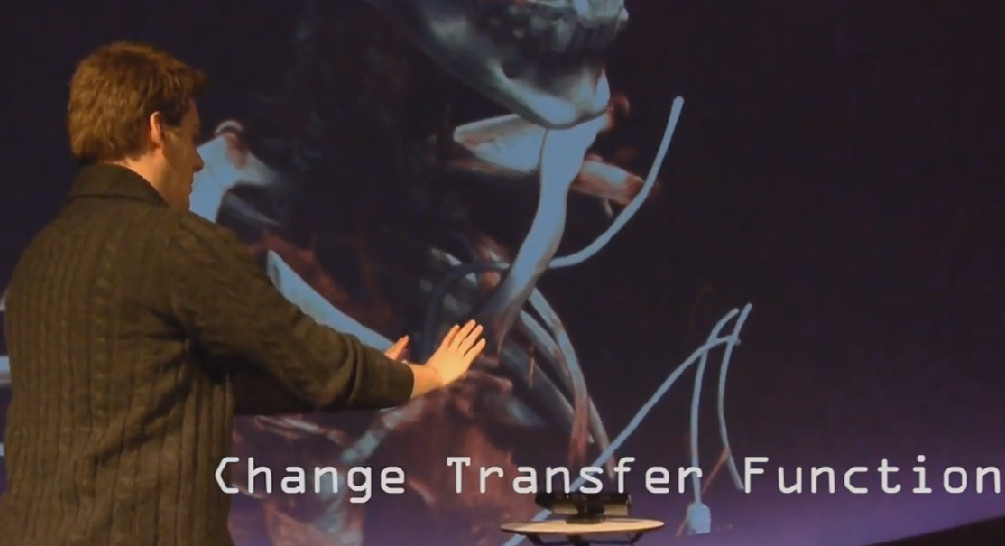
\includegraphics[width=1.0\linewidth]{images/dome_tf_change}}
%	\caption{Dome Closeup}
%	\label{img:dome_tf_change}
%\end{figure}

%% These three lines bring in essential packages: ``mathptmx'' for Type 1
%% typefaces, ``graphicx'' for inclusion of EPS figures. and ``times''
%% for proper handling of the times font family.

\usepackage{mathptmx}
\usepackage{graphicx}
\usepackage{times}
\usepackage{amsmath}
\usepackage{flushend}
\usepackage{subfigure}
\usepackage[noabbrev]{cleveref}
\usepackage{color}
%\usepackage[caption=false]{subfig}
\setlength{\fboxsep}{0pt}
\newcommand{\todo}[1]{\textbf{\textcolor{red}{[TODO: {#1}]}}}

%% We encourage the use of mathptmx for consistent usage of times font
%% throughout the proceedings. However, if you encounter conflicts
%% with other math-related packages, you may want to disable it.

%% This turns references into clickable hyperlinks.
%%\usepackage[bookmarks,backref=true,linkcolor=black]{hyperref} %,colorlinks
%%\hypersetup{
%%  pdfauthor = {},
%%  pdftitle = {},
%%  pdfsubject = {},
%%  pdfkeywords = {},
%%  colorlinks=true,
%%  linkcolor= black,
%%  citecolor= black,
%%  pageanchor=true,
%%  urlcolor = black,
%%  plainpages = false,
%%  linktocpage
%%}

%% If you are submitting a paper to a conference for review with a double
%% blind reviewing process, please replace the value ``0'' below with your
%% OnlineID. Otherwise, you may safely leave it at ``0''.
\onlineid{0}

%% declare the category of your paper, only shown in review mode
\vgtccategory{Position Paper}

%% allow for this line if you want the electronic option to work properly
\vgtcinsertpkg

%% In preprint mode you may define your own headline.
%\preprinttext{To appear in an IEEE VGTC sponsored conference.}

%% Paper title.

\title{An audience-centric view of interaction techniques in interactive presentations of scientific 3D data}

%% This is how authors are specified in the journal style

%% indicate IEEE Member or Student Member in form indicated below
%% indicate IEEE Member or Student Member in form indicated below
%\author{Erik Sund\'en, \textit{Member, IEEE}, Alexander Bock, \textit{Student Member, IEEE}, Daniel J\"onsson, \textit{Student Member, IEEE}\\ and Timo Ropinski, \textit{Member, IEEE}}
%\authorfooter{
%% insert punctuation at end of each item
%\item
% Erik Sund\'en, Alexander Bock, Daniel J\"onsson and Timo Ropinski are with Link{\"o}ping University. E-mail: \{erik.sunden,alexander.bock,daniel.jonsson,timo.ropinski\}@liu.se.
%}

\author{Erik Sund\'en\thanks{e-mail:erik.sunden@liu.se}\\ %
        \scriptsize Link{\"o}ping University %
\and Alexander Bock\thanks{e-mail:alexander.bock@liu.se}\\ %
			   \scriptsize Link{\"o}ping University %
\and Daniel J\"onsson\thanks{e-mail:daniel.jonsson@liu.se}\\ %
          \scriptsize Link{\"o}ping University %
\and Timo Ropinski\thanks{e-mail:timo.ropinski@liu.se}\\ %
           \scriptsize Link{\"o}ping University }


%other entries to be set up for journal
%\shortauthortitle{Sund\'en \MakeLowercase{\textit{et al.}}: Hands-only 2D vs 3D interaction when exploring volume data}
%\shortauthortitle{Firstauthor \MakeLowercase{\textit{et al.}}: Paper Title}

%% Abstract section.
\abstract{ 
In this paper we share our experiences with different types of interaction, such as 2D direct touch and 3D tracking, in various scenarios and environments which involve not only a user, but an audience, with a novice level of expertise in the area of interaction within scientific visualization. Our focus is on describing ways of interacting with the data, with the focus on how natural and understandable they are for the audience. While some natural exploratory interaction methods fit well for the user, they may be less beneficial when presenting the data to the audience. Of course, an appropriate natural interaction for the user can in many scenarios be an appropriate interaction for the audience, but our observations show that it usually highly dependent on the setting where the interaction and viewing takes place.
} % end of abstract

%% Keywords that describe your work. Will show as 'Index Terms' in journal
%% please capitalize first letter and insert punctuation after last keyword
\keywords{interaction, audience, 2D, 3D, touch display, kinect, voice}

%% ACM Computing Classification System (CCS). 
%% See <http://www.acm.org/class/1998/> for details.
%% The ``\CCScat'' command takes four arguments.

%\CCScatlist{ % not used in journal version
%   \CCScat{I.3.7}{Computer Graphics}{Three-Dimensional Graphics and Realism}{Color, shading, shadowing, and texture}
%}

%% Uncomment below to include a teaser figure.
%  \teaser{
%  \centering
%  \includegraphics[width=16cm]{CypressView}
%  \caption{In the Clouds: Vancouver from Cypress Mountain.}
%  }

%% Uncomment below to disable the manuscript note
%\renewcommand{\manuscriptnotetxt}{}

%% Copyright space is enabled by default as required by guidelines.
%% It is disabled by the 'review' option or via the following command:
% \nocopyrightspace

%%%%%%%%%%%%%%%%%%%%%%%%%%%%%%%%%%%%%%%%%%%%%%%%%%%%%%%%%%%%%%%%
%%%%%%%%%%%%%%%%%%%%%% START OF THE PAPER %%%%%%%%%%%%%%%%%%%%%%
%%%%%%%%%%%%%%%%%%%%%%%%%%%%%%%%%%%%%%%%%%%%%%%%%%%%%%%%%%%%%%%%%

\begin{document}

%% the only exception to this rule is the \firstsection command
%\firstsection{Introduction}\label{sec:introduction}

%% The ``\maketitle'' command must be the first command after the
%% ``\begin{document}'' command. It prepares and prints the title block.
\maketitle

\section{Introduction}\label{sec:introduction}
Different types of interaction within visualization have in recent years become increasingly common due to the introduction of low-cost interaction devices.
Since a couple of years it is no longer obvious that a mouse and keyboard will be used as the main type of interaction. 
Touch screens are now de-facto standard for phones and tablets while low-cost solutions for touchless interaction, such as the Kinect, has inspired a range of applications. 
Much focus has been on the level of interaction expertise of the user to determine if the type of interaction is suitable for a certain scenario.
However, the intended use of the application and the place where it is located are also of great importance. \todo{This needs a better transition (ab)}

An analogy can be made with the visualization community, which commonly classifies the use of visualization into exploration, analysis and presentation. 
Each usecase typically requires a different approach and tools. 
While the exploration phase requires a flexible interaction with the visualization, 
the presentation phase is scaled down to allow the user to change only a few parameters or for example use a pre-determined animation.\todo{The 'why is this so' is quite important at this point (ab)}
This distinction has to our knowledge not been done for interaction and we will in this manuscript focus on the use of interaction for presentation purposes. 
This involves one or more people interacting with a visualization in order to present information to an audience that may consist of a single person or many people.
What has not recieved much attention before is that the type of interaction used also affects the impact of the presentation and is therefore also part of it. 
If the audience can infer what will happen by the interaction it could help them follow the flow of the presentation. \todo{This needs a much stronger focus (ab)}

We will draw examples from scientific visualization where the presenter is not simply switching slides but is trying to tell a story about the data being visualized. \todo{Example (ab)}
Typical parameters that are altered include the moving the camera (i.e. rotate, translate and zoom), cropping the data set in order to reveal information inside and applying different type of filters such as a threshold to hide undesirable information. \todo{Do classes of interaction methods exist, rather than giving examples? (ab)}
We will show examples on how these parameters can be changed for touch and touchless interaction and discuss our experience in using them in different settings, with respect to size of screen and audience, for presentation purposes. \todo{Which parameters? (ab)}
%While we comment on expert viewers, the focus this paper is on none expert viewers, together with either an expert or none expert user. Our definition of expert is a person which is familiar within the area of volume data exploration.
%
%....Touchless 3D interaction (kinect) vs touch screen 2D interaction....different scenarios such as slicing, clipping, zooming in 2D and 3D visualization of medical volume data.
%\todo{Point out: Interaction is part of the presentation}

Using an object such as a mouse, can be useful both in 2D and 3D movements.

If the user has training with a certain device coupled with a specific application, the expert user may certainly benefit from the type of interaction instead of hands-only interaction. \todo{I would leave this out completely as it does not matter to the content of presentation (ab)}

However, for a none expert, which is the focus of this paper, a mouse/joystick offers unnatural ways of exploring the scientific data, as the hands are not directly interacting with the visualization of the data. \todo{Again, we don't consider the "naturality" of the interaction (ab)}

Mouse vs Kinect vs Leap vs Myo \cite{doi:10.1117/12.2006994}. \todo{I would like to see a paragraph somewhere saying that the actual technology does not matter for the interaction, as there is no big difference between a kinect or a leap motion, for example. (ab)}

Natural of touchless \cite{O'hara:2013:NTP:2442106.2442111}

Volume Cracker (3D interaction with gadgets) \cite{Laha:2013:VCB:2491367.2491368}

\section{(Daniel) Scenario: Single user exploration}

This scenario deals the situation when the presentation is performed on a small screen, such as a tablet or desktop monitor, and the audience consists of a few people. 
The distance between the audience and the presenter is typically small and allows for a tight communication between the two parts. 
The audience can easily communicate preferences in what to explore and may in some cases even intervene with the presenter to interact with the visualization. 
An intuitive interaction can therefore engage the audience and create a more dynamic presentation.
An example can be seen in~\cref{img:touch_workstation}, where the presenter uses a touch screen to interact with a fetus scanned using ultrasound.
The presenter can in this case switch to different modes, which controls the behaviour of the gestures. 
The standard mode rotates, translates and zooms using single finger, two fingers moving together and pinching, respectively. \todo{Or other gestures... More general? (ab)}
Switching to transfer function mode will change the interpretation of the single finger touch such that the threshold and opacity are changed according to the horizontal and vertical movement. \todo{At this point, what is the transfer function mode? Why is switching necessary at all? (= simplifying interaction design) (ab)}

%This scenario deals with small screens and 
%User-centered...
%
%Mouse can be relevant, as touch devices.
%
%Touch good, reaching to the data. Especially when the user in question is not an expert in handling connected devices in that specific scenario.
%
%Clipping, 2D to 3D representation of region.
%
%Rotation, gripping points.

\begin{figure}[htb]
	\centering
	\fbox{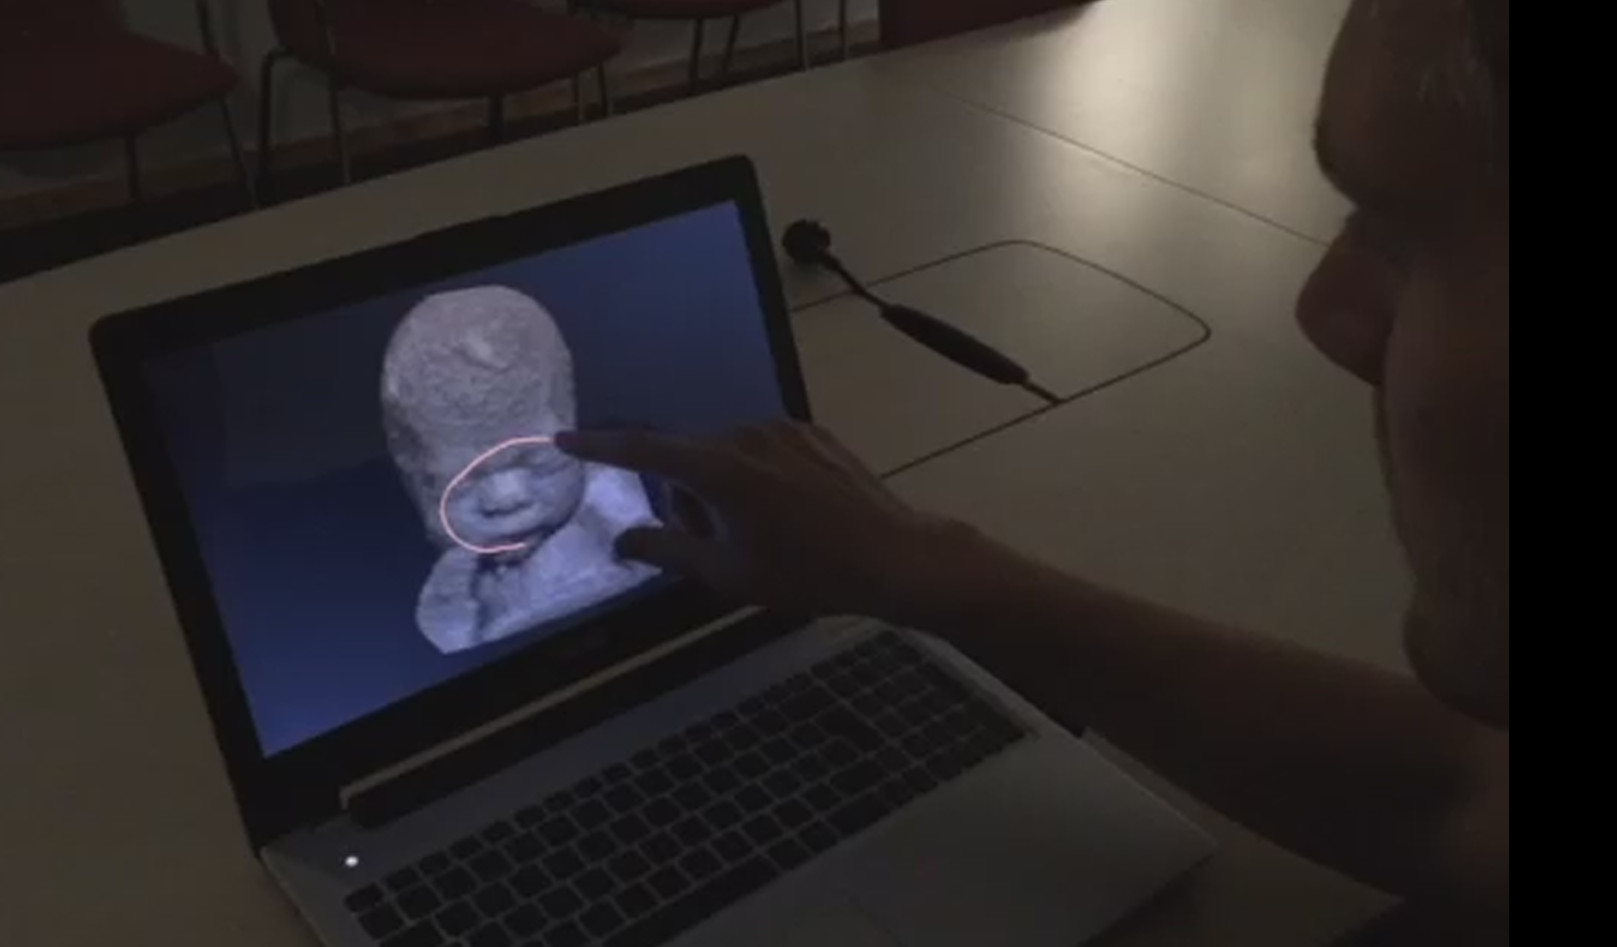
\includegraphics[width=1.0\linewidth]{images/touch_workstation}}
	\caption{Visualization of a fetus scanned using ultrasound. Touch screen interaction is used to change camera, transfer function and clipping.}
	\label{img:touch_workstation}
\end{figure}

\section{(Erik) Scenario: Exhibition Area}

In an exhibition area there is often both small to medium sized displays utilized to showcase and explore the scientific data. Furthermore, there is mostly none experience users and viewers present which interact and view others interact with the scientific data. There are a wide range of setups with certain displays and gadgets for immersive and exploratory purposes which can be utilized in an exhibition area, such as \cite{Laha:2013:VCB:2491367.2491368} \todo{More references}. What they all have in common when it comes to this scenario is that naturalness of the interaction is highly important \todo{Explain why? (ab)}. That fact, together with a reasonable level of functionality motivates the usage of hands-only setup, trough direct touch \cite{Klein:2012:DSD:2322389.2322403} and touchless methods \cite{O'hara:2013:NTP:2442106.2442111}.

In figure \ref{img:exhibition_table} we see an exhibition setup example, known as an autopsy table \cite{LRFPY11}, where data such as a CT scan of a human can be explored in a close to true scale environment, using direct touch and multi-touch gestures. Rotation of the object is done with a one finger trough an up and down movement, translation is performed with a one finger side-to-side sweeping and zoom with a two-finger pinch gesture.

In a sense it is just an increased version of a tablet, but suitable for a larger audience, as the area surrounding the table is significantly larger. With this in mind, the naturalness of the interaction for the user would benefit from as close to real life movements as possible, to support the true scale visualization. This is of course a challenge for direct touch displays, as there is a 2D instead of a 3D user experience. However, it can be considered a commonly known practice how to interact with touch displays, trough common gestures such as pinch and swipe. As high-resolution accurate touch screens are available today, this type of setup is very appreciated for both the user and the audience.
\todo{What are the implications of the small/large touch devices? (ab)}

\begin{figure}[htb]
	\centering
	\fbox{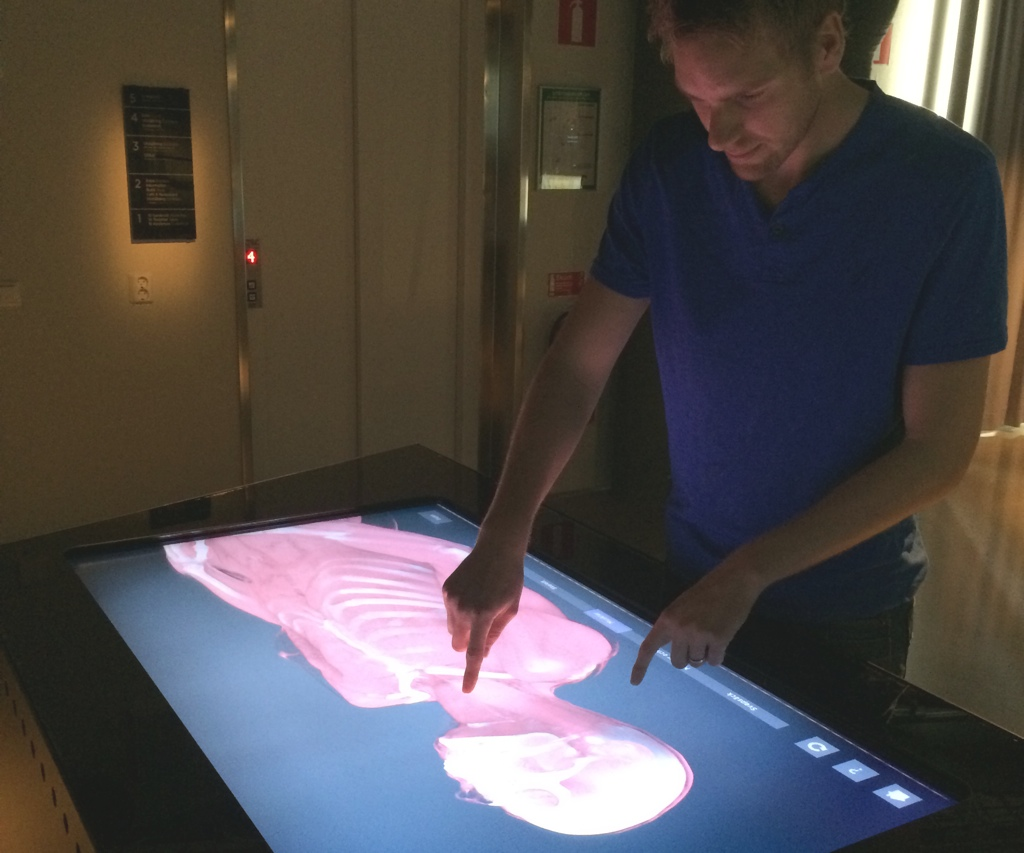
\includegraphics[width=1.0\linewidth]{images/exhib_table}}
	\caption{A touch table (known as the Autopsy Table) for scientific data exploration of for instance scans of humans or animals which can be viewed in close to true scale.}
	\label{img:exhibition_table}
\end{figure}

The setup in figure \ref{img:exhibition_kinect} is similar to figure \ref{img:exhibition_table} in terms of exploring data in true scale. The difference lie in the display surface, which is now without 2D interaction trough direct touch, and instead coupled with 3d interaction trough hand tracking \todo{How is this interaction 3D? (ab)}. This setup can support a larger audience due the shear placement of the display surface, but comes with the downsides of a decoupled user interaction experience. The user will feel less in control of the data, even if you neglect the accuracy of the tracking, because he is not directly touching the display surface. Furthermore, the interaction might be less natural then direct touch, and the gestures more comprehensive to support the same level of functionality \todo{I don't get this sentence (ab)}. For instance, in our setup one hand is used for manipulating the camera or the light source, while the second hand acts as a state changer which tells the program what the moving hand should be mapped to \todo{Refer to "Why states" above (ab)}.

As seen in figure \ref{img:exhibition_kinect}, a hand cursor is rendered which simulates the projection of the users hand onto the surface. Such visual cues not only help the user, but also allow a wider understanding for the audience to comprehend what operation the user is currently performing \todo{How is that achieved? (ab)}. Furthermore, the icons in the bottom are not only introduced to avoid a increase in the quantity and complexity of gestures for different operations, but also to make the operations performed more in contact with the visualization \todo{That needs some argumentation; before, the baseline is: gestures are good since natural, now we argue that icons are better than gestures (ab)}.

When comparing observations from the direct-touch and the touchless setup the visual cues in the touchless setup has so large impact for the novice user and viewer, when it comes to gestures, but only if the gestures are projected onto the screen in a natural way \todo{I don't get this (ab)}. It can also be noted, that these type of visual cues are not easily introduced into the touch table to increase the level of comprehension for the interaction, as all natural projection of for instance the users hands would be blocked by the hands themself \todo{I find this paragraph very confusing, I don't understand what you mean (ab)}.

\todo{Develop this further in Large Audience section with the rendering of 3D arms....}

\textbf{Conclusions:}
Based on our observations we conclude that when performing a limited amount of operations, the setup with projector and 3D hand tracking is more optimal then the touch screen coupled with 2D finger gestures, when it comes to how the audience perceive the effect of interaction onto the visualization \todo{Do we? I thought it was a function of audience size? (ab)}. The reason for this is that both the visualization and the projection of interaction can be visualized and perceived by the audience onto the display. This is not possible in practice if the user would directly interact with the display surface, as the projection of the users movement would be blocked by his hands, both for the audience and the user \todo{This only holds true for small display sizes, ratio hand size/screen size (ab)}.

\begin{figure}[htb]
	\centering
	\fbox{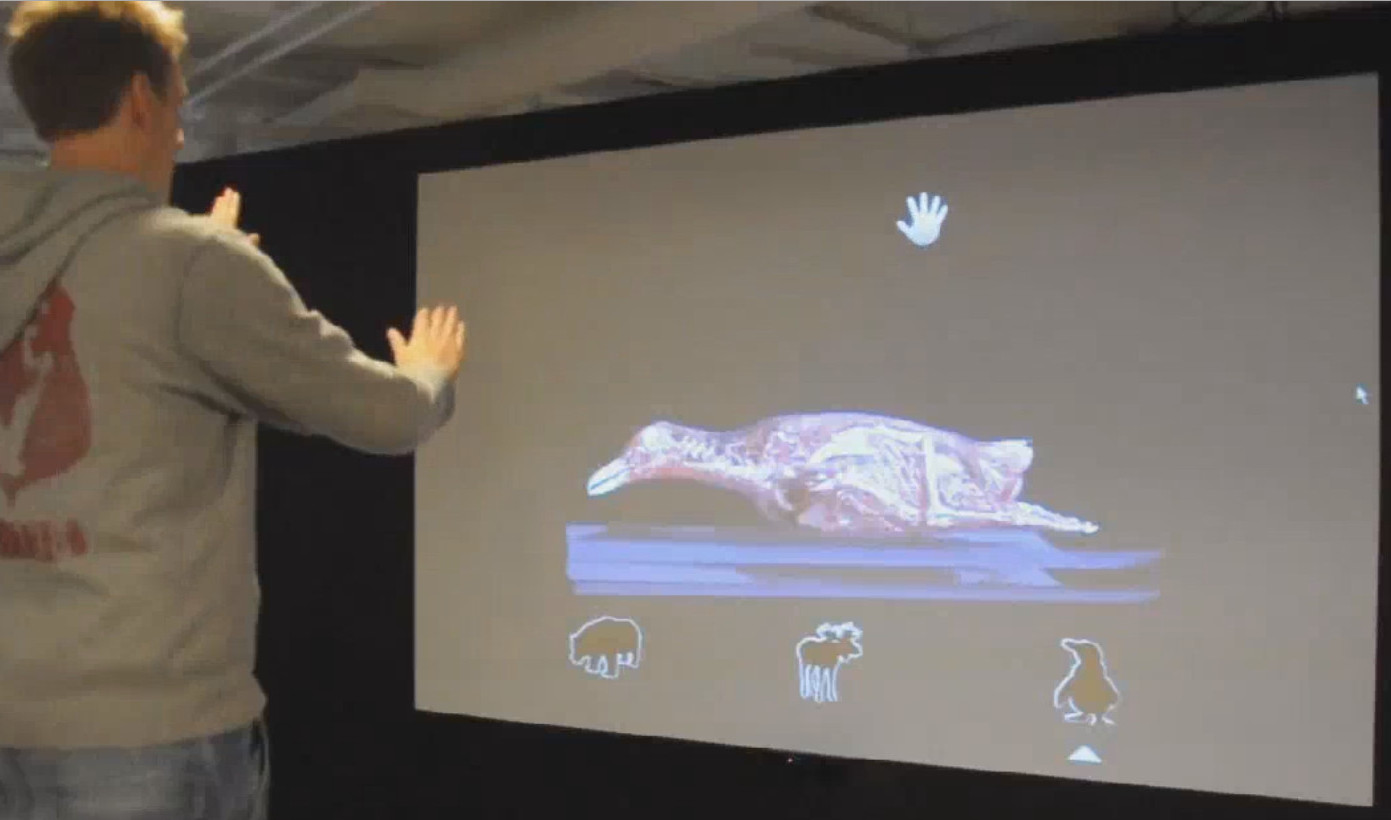
\includegraphics[width=1.0\linewidth]{images/exhib_rotate_peng}}
	\caption{Volume visualization of a CT scanned penguin displayed on a wall with a in-front projector and coupled with a kinect for 3D interaction possiblities.}
	\label{img:exhibition_kinect}
\end{figure}

...

\section{(Alex) Scenario: Large Audience Presentation}

\noindent \textbf{Oral Presentation} Being the most traditional form of 1 to many presentation techniques, oral presentations have been around since time immemorial.
While they were restricted to a lecturer talking to the audience in the beginning, over time more and more tools and techniques have been added to improve the information transfer to the audience.
Adding a blackboard allows the presenter to construct a visual representation of the information he is conveying while he is explaining the subject matter.
In these early forms, the audience is witness to the construction and can follow the construction as it happens, thus increasing the knowledge transfer as compared to after-the-fact representations [citation needed].
Nowadays, the blackboard has been replaced with a whiteboard or alternatively a slide presentation, but the fundamental principle has not changed since the beginning.
This can be seen in the fact that must slide shows still follow the tradition of constructing the explanations in a linear form and are fairly standardized for each field [citation from Vis 2012].

A prime example of an enhanced oral presentation technique in which the interaction technique matters a great deal is medical schools' education based on cadavers.
In these settings, a lecturer dissects a cadaver live in front of students in order to teach them about a specific subject of the human body.
Here, not only the content is of importance to the audience, but also the individual steps of how the presenter interacts with the body as this is one of the foci of study.
While the previous example supports, in theory, an unlimited audience size, the medical example is limited by the fact that every audience member has to see the presenter and cadaver.
We found that this simple restriction is present in many interaction techniques that we investigated.
Being able to see and understand the movements and gestures of the presenter is important for understanding the information that is conveyed.
This medical example is a good example of the necessary trade-off between interaction design, audience size, and the possibility of using large-scale displays as a presentation tool.

The next logical development step for large-scale, large-audience display scenarios is to include interactive, rather than predetermined, content content.
The results of the discussion for this scenario are independent of the data that is shown or the details of the interaction, as the first-order approximation of the usage scenario is the same.
Principally, we can distinguish two classes of solutions for this interaction problem.

The first class, being direct interaction, requires the lecturer to perform the interaction himself.
The availability for this kind of interaction is heavily dependent on the screen-size and the layout of the venue.
For a detailed discussion of this class of solution, see below [or where ever].

The second class is indirect interaction (see Figure~\ref{img:dome_presentation}), where the lecturer is communicating orally with a second person controlling the visualization and thus content.
For this part, we assume that the audience hears the communication between the two people.
From an interaction point of view, this interplay between presenter and controller has both benefits and drawbacks.
One benefit is the added dynamics between the presenter and the controller, creating a more dynamic environment for the audience compared to just listening to the presenter, which creates a more engaging environment, itself sparking more interaction between the audience and the presenter.
From an interaction point of view, the audience is witness to the intended action of the interaction, rather than the physical act of interacting itself.
The audience knows that, for example, the focus will be on a specific part of a rendering before it happens.
Rather than being witness of the manual interaction leading to that focus, it perceives the interaction as being completely indirect and decoupled from the presenter.
By removing any signs of an interaction, the visualization seems more seamless and the presenter can focus on the presentation and content rather than multitasking with the presentation and the controlling.
The explicit details of the interaction in this case fall outside the scope of this paper, as the audience will not (in general) see how the controller interacts with the visualization.
This decoupling is the prime attribute for this class of interaction solutions and whether this is a benefit or drawback depends on the situation to which it is applied.

A slight variant to this is the concept of remote presentations.
In this case, the presenter is not in the same room as the intended audience, but his voice (and possible video footage) is streamed live into the same room.
From an interaction point of view, this does not change much, as the presenter's interaction with the content was limited to a oral communication with the controller.
This interaction is completely unchanged in this variation.
The only visible difference to the audience is the missing presence of the presenter in the same room.
An increase in presence techniques, such as 3D conference applications, will in the future further blur the line between a physically-present presenter and a remote presenter.


\noindent \textbf{Dome vs VR Arena vs Decision Arena} In our research facility, we have access to three different display devices that bear superficial similarities, but induce fundamental differences in how the interaction with the visualization and interplay with the audience works.

One of the display systems is a 160 degree field-of-view hemispherical dome surface with seating for 99 audience members, which is projected on using a stereo projector system.
This is a similar setup to the ones used in traditional planetariums, but in our case, an interactive rendering system is used instead to produce the content.
The interaction characteristics for this setup is that both the audience and the presenter are at a great physical distance (usually > 5 meter) from the projection surface.
This completely inhibits direct interaction techniques like pointing with a finger or doing gestures that are directly relate to the content that is shown on the screen.
Instead, indirect techniques must be used, like laser pointers, rendered cursors on the screen, gesture recognition, or oral communication with a controller.
One issue with this system is the impossibility of mapping physical gestures to match the visualizations.
Due to the large scale of the room and the wide differences in seating position, it is not possible to place the presenter in such a way that his gestures would seem integrated into the visualization for all viewers simultaneously.

The other setup available onsite is a flat, back-projected surface using three full HD projectors, which are aligned to produce a wide projection surface of about 5000$\times$1080 pixel [check with Miro].
The room in which this is located seats about 30 people.
The benefit of having a back-projection is that the presenter can stand in front of the projection without casting a shadow on the projection surface, thus allowing physical access to the displayed content.
In comparison to the dome theater, this, and the limited size, allows the presenter to walk in front of the whole content and using natural gestures like pointing (which may be integrated, registered, and synchronized with the rendering) to interact with the content.
This natural, gesture-free interaction has been proved very useful in the workflow that we use in the facility.

The third setup is a curved-screen decision arena in which the audience members are located on the inside of a round room with the walls being used as projection surfaces.
This setup is very useful for a small group of people ($<$ 10 persons) to simultaneously work on decisions using the information projected on the surfaces.
The interaction techniques for this, as compared to the previous two, are fairly limited in regular usage, as this is not a tradition presentation setup, but rather a collaborative exploration of data using visualization.


\begin{figure}[htb]
	\centering
	\fbox{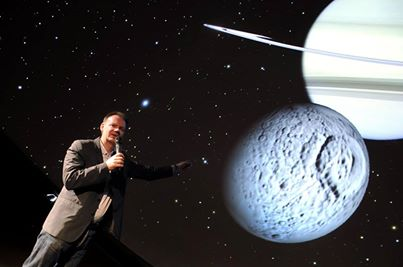
\includegraphics[width=1.0\linewidth]{images/dome_oralpresentation}}
	\caption{Presentation on large scale surfaces}
	\label{img:dome_presentation}
\end{figure}

\begin{figure}[htb]
	\centering
	\fbox{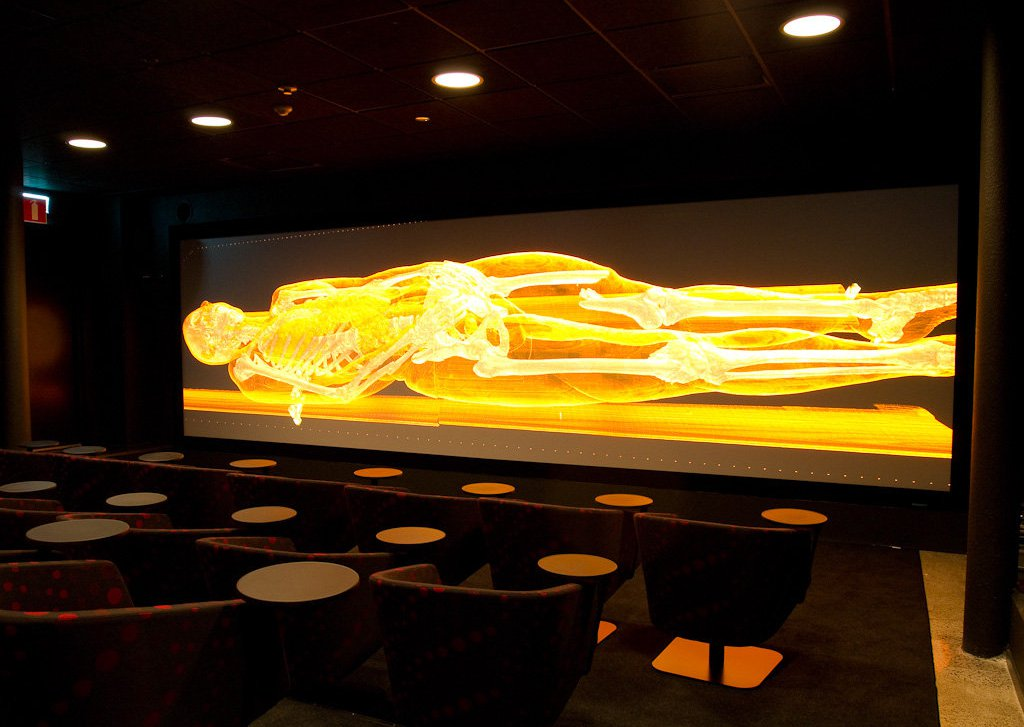
\includegraphics[width=1.0\linewidth]{images/vr_dvr}}
	\caption{A volume rendering on a flat, back-projected surface}
	\label{img:vr_dvr}
\end{figure}


%Presenter is always decoupled from the screen, as the presenter can not interact with the complete presentation surface. This is often due to the lack of touch capability, but foremost the sheer size of common screens for large audience presentations can not be reached from a standing location by the user.

%Dome, movement, viewers benefit to see how presenter interacts with the data.
%Thus, big 3D gestures better then gesture on touch device.

%User should be standing in such away that the 3D movements the user performs can be projected correctly onto the screen.

%Discuss interaction option made by audience, pros and cons


\begin{figure}[htb]
	\centering
	\fbox{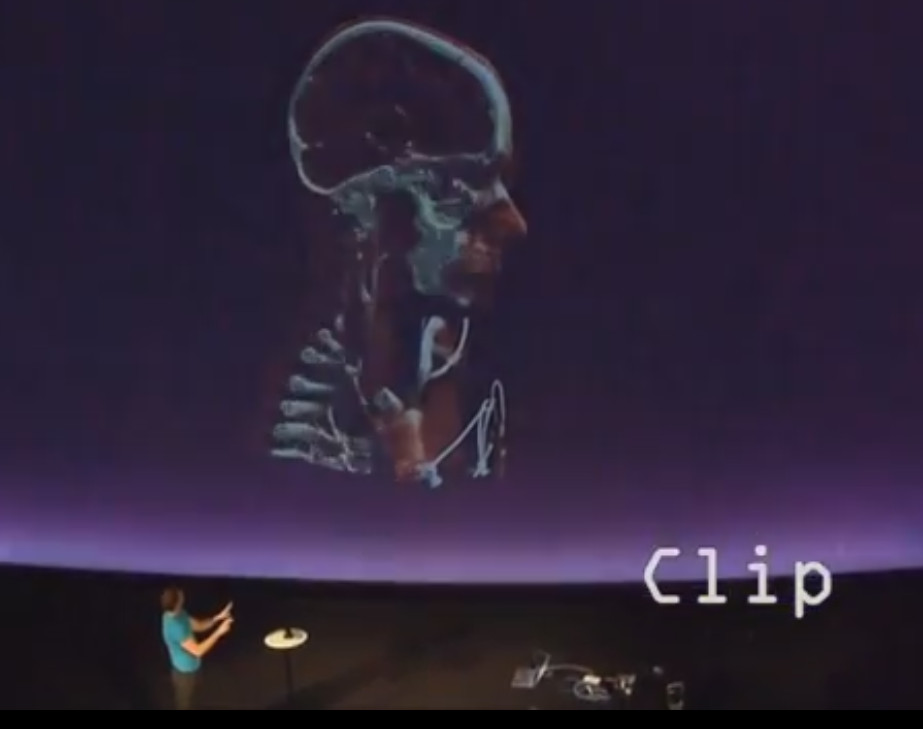
\includegraphics[width=1.0\linewidth]{images/dome_clip}}
	\caption{Dome}
	\label{img:dome_clip}
\end{figure}

\begin{figure}[htb]
	\centering
	\fbox{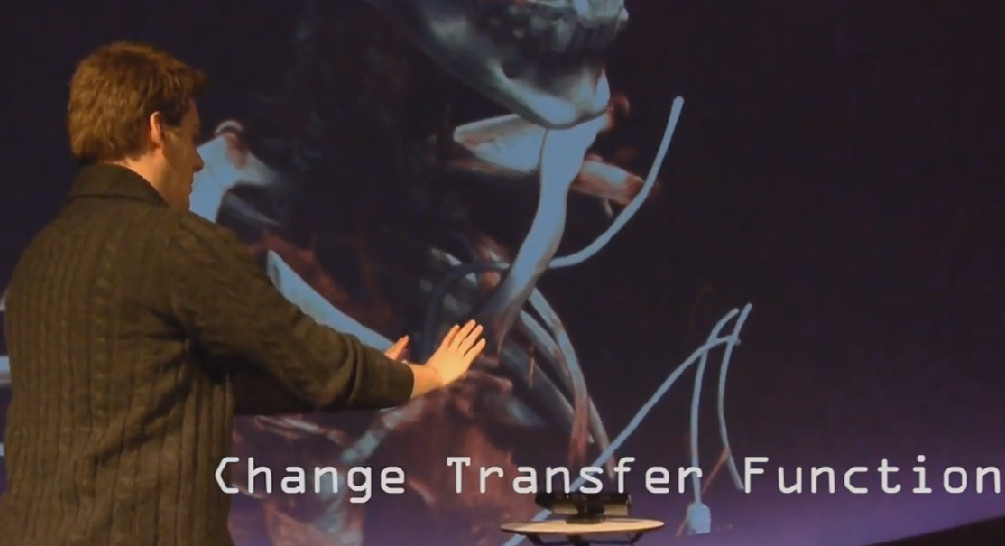
\includegraphics[width=1.0\linewidth]{images/dome_tf_change}}
	\caption{Dome Closeup}
	\label{img:dome_tf_change}
\end{figure}

\section{Interaction techniques from the scenarios}

So far, not every possible technique suited for the scenarios is covered. However, finding the most suitable technique for our different scenarios is not the focus of our position paper, but rather we propose a way to think about interaction methods dependent on the scenario. In this section we summarize the method of interaction which are part of our previously described scenarios.

\subsection{Direct Touch Interaction}
Direct interaction with an object in the scene gives the user a feel of control of the object~\cite{isenberg2009studying}. 
The user touches the screen and the 2D motion is mapped to a 3D manipulation of the object. 
Touch interaction in scientific visualization has not received much attention in the past \cite{isenberg:hal-00781512}, 
but more work is starting to appear~\cite{Klein:2012:DSD:2322389.2322403} and it has already been used in applications~\cite{LRFPY11}.
From a presentation perspective the audience can see the movements of the presenter and thereby get an understanding of what will happen on the screen.
However, the presenter will also hide part of the screen due to the occluding hands and arms. 
When the audience grows larger it may be hard to see the gestures and the benefit of seeing the presenter's movements decreases.

%Importance of Touch \cite{Robles-De-La-Torre:2006:IST:1158827.1159097}

\subsection{Touchless Interaction}

Kinect dicom \cite{zora82163}

Kinect operation \cite{OHaraGSPVMCCRDC14}

Interactive Slice WIM \cite{Coffey:2012:ISW:2360744.2360843}

Touchless surgery \cite{Mentis:2012:IPI:2207676.2208536}

Touching the 3rd dimension \cite{DBLP:journals/dagstuhl-reports/KeefeKSR12}

\subsection{Gestures}

Evaluation of Gesture \cite{Kirmizibayrak:2011:EGB:2087756.2087764}

Discuss gesture vs postures \cite{isenberg:hal-00781237} for kinect, and gesture available for both touch and kinect.

\subsection{Voice}

\section{Classification}

To further show when a certain interaction technique is preferable from an expressiveness to audience point of view we introduce a classification of the techniques covered in our scenarios. The chart show the relevance of the technique in relation to audience and display size. It should be noted, that while a technique usage relevance is highly dependent on the scenarios and might be less suitable in when it comes to different scenarios.

\begin{figure}[htb]
	\centering
	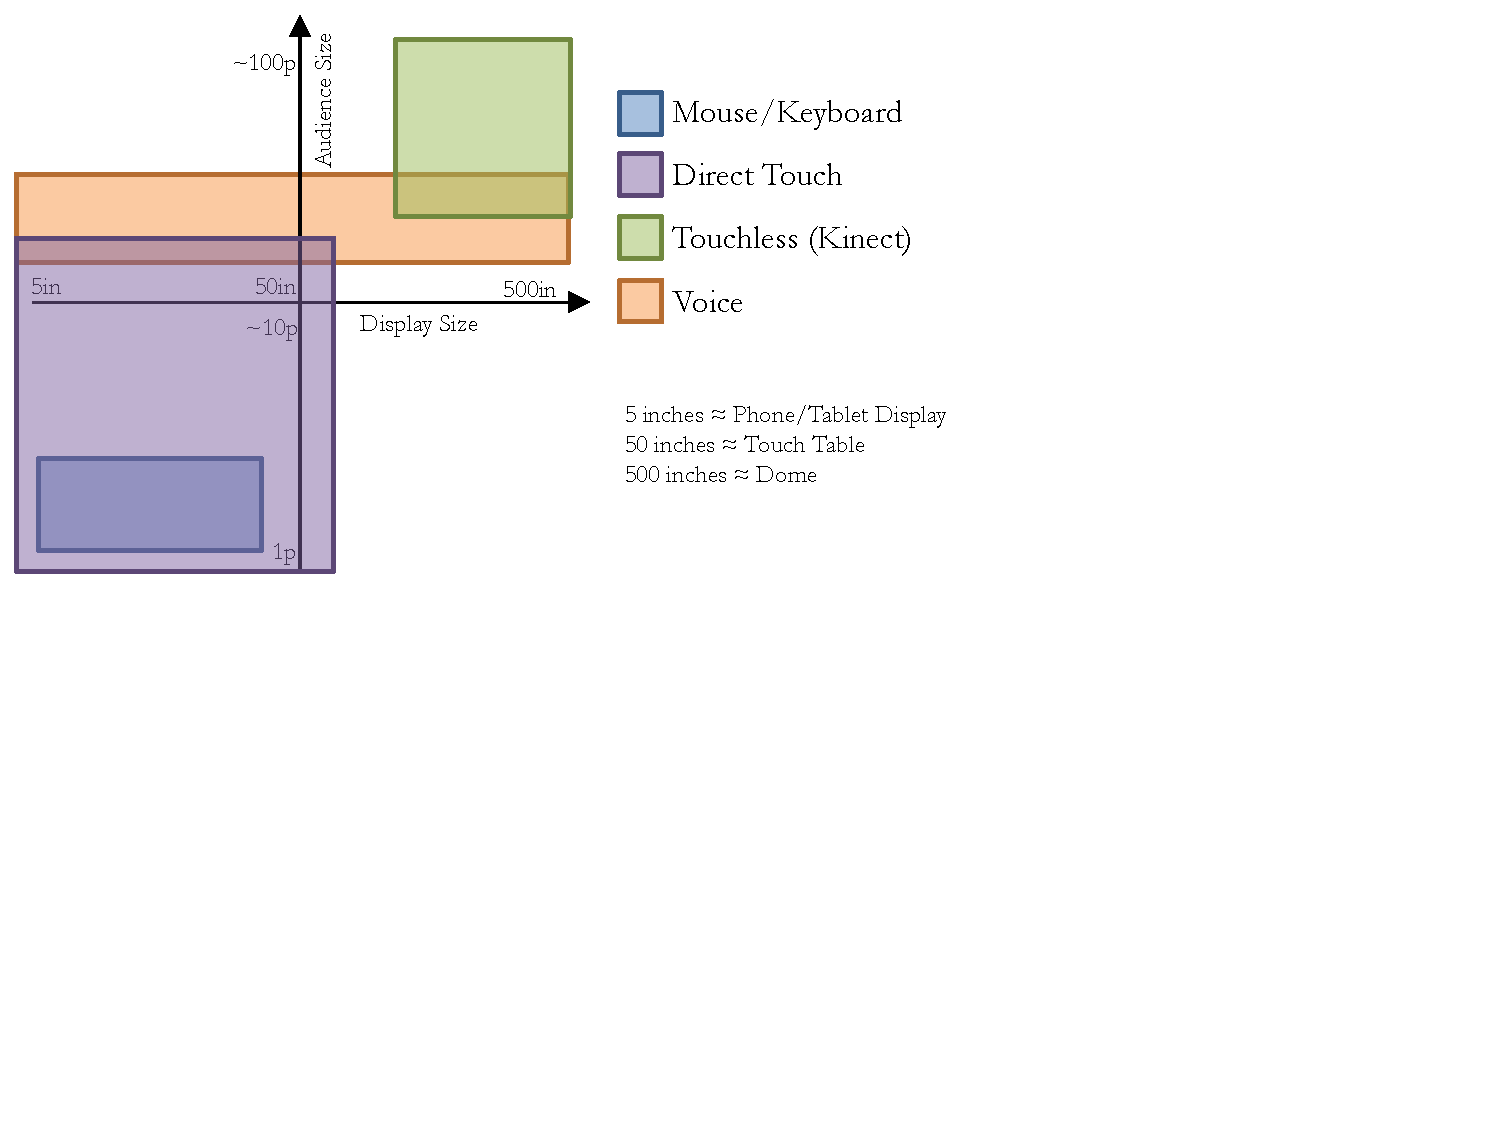
\includegraphics[width=1.0\linewidth]{classifiy_diagram.pdf}
	\caption{Relevance chart mapped to technique categories and our situations.}
	\label{classifiy_diagram}
\end{figure}

There are more advanced classification methods for interaction techniques, especially for 3D user interaction \cite{Kettner95aclassification}, but there focus cover the usability for the actual user.

\section{Conclusions}\label{sec:conclusion}

There is no surprise that a decoupled interaction approach is often less intuitive then one which the viewing surface and interaction area is the same.
However, when a decoupled approach is necessary certain elements can be introduced in order to help the audience.
Such as projecting the hand onto the viewing surface.

\todo{Emphasize that simple voice commands can be introduced as complementary to 3D tracking to lower the needed complexity of the gestures}

With this paper we wanted to share our observations about interaction as presentation tool and we deem that an the research within viewer or audience centered interaction methods should receive more attention. We strongly encourage researchers within 2D and 3D user interaction interfaces to include this aspect when evaluating previous and future techniques.
Within this subject, expert and none expert viewers have different ways of thinking and experiencing data exploration. Thus, the naturalness of the interaction could does be completely different for the different viewers.

\bibliographystyle{abbrv}
%%use following if all content of bibtex file should be shown
%\nocite{*}
\bibliography{literature}
\end{document}
